\documentclass[border=4pt]{standalone}
\usepackage[T1]{fontenc}
\usepackage{lmodern}
\usepackage{amsmath}
\usepackage{pgfplots}
\pgfplotsset{compat=1.18}
\usepgfplotslibrary{groupplots,fillbetween}
\usetikzlibrary{calc,arrows.meta}
% one colour per kind of method, the same in every figure (Okabe-Ito)
\definecolor{neur}{HTML}{D55E00}   % neurons chosen by attribution
\definecolor{dirc}{HTML}{009E73}   % directions from the weird-vs-normal contrast
\definecolor{read}{HTML}{0072B2}   % readout methods and interventions chosen from readouts
\definecolor{pers}{HTML}{CC79A7}   % Assistant Axis / persona
\definecolor{ctrl}{HTML}{8C8C8C}   % random controls
\definecolor{meas}{HTML}{E69F00}   % measured outcome
\definecolor{ink}{HTML}{222222}
\pgfplotsset{
  every axis/.append style={clip=false, font=\small, axis line style={black!55}, tick style={black!55}, tick align=outside,
    label style={font=\small}, tick label style={font=\footnotesize}, title style={font=\small, align=center}},
  grid style={black!9, line width=0.4pt},
  every axis legend/.append style={font=\footnotesize, draw=none, fill=none},
  ci/.style={/pgfplots/error bars/x dir=both, /pgfplots/error bars/x explicit, /pgfplots/error bars/error bar style={line width=0.8pt}, /pgfplots/error bars/error mark=none},
  yci/.style={/pgfplots/error bars/y dir=both, /pgfplots/error bars/y explicit, /pgfplots/error bars/error bar style={line width=0.8pt}, /pgfplots/error bars/error mark=none},
}

\begin{document}
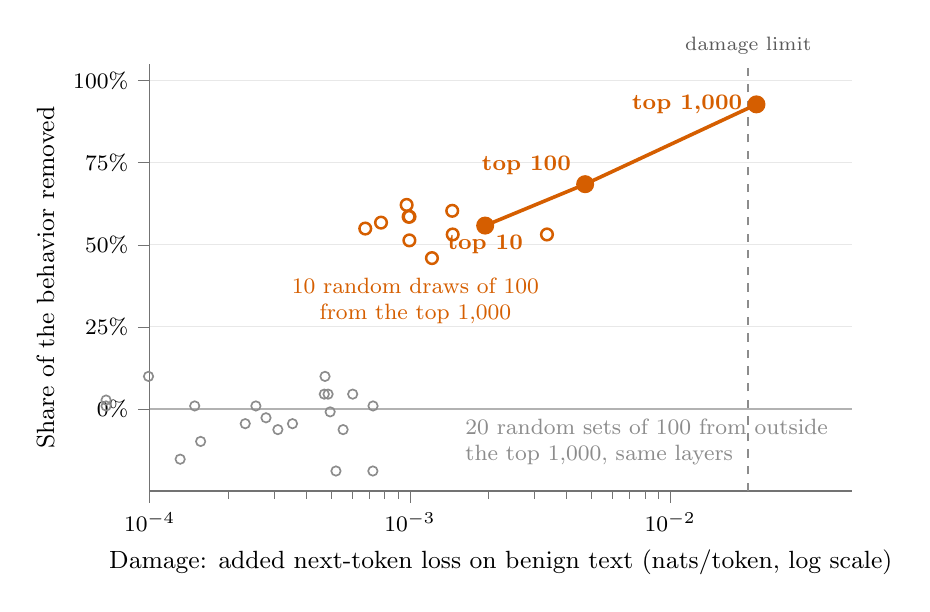
\begin{tikzpicture}
\begin{axis}[width=10.5cm, height=7cm, xmode=log, xmin=1e-4, xmax=0.05, xtick={1e-4,1e-3,1e-2}, xticklabels={$10^{-4}$,$10^{-3}$,$10^{-2}$}, ymin=-25, ymax=105, ytick={0,25,50,75,100}, yticklabel={$\pgfmathprintnumber{\tick}\%$}, axis x line*=bottom, axis y line*=left, ymajorgrids, xlabel={Damage: added next-token loss on benign text (nats/token, log scale)}, ylabel={Share of the behavior removed}]
\draw[black!30, line width=0.5pt] (axis cs:1e-4,0) -- (axis cs:0.05,0);
\draw[black!45, dashed, line width=0.7pt] (axis cs:0.02,-25) -- (axis cs:0.02,105) node[anchor=south, font=\scriptsize, black!65] {damage limit};
\addplot[only marks, mark=o, mark size=1.7pt, ctrl, line width=0.6pt] coordinates {(0.000233,-4.50) (0.000472,9.91) (0.000068,2.70) (0.000722,0.90) (0.000256,0.90) (0.000068,0.90) (0.000157,-9.91) (0.000494,-0.90) (0.000311,-6.31) (0.000354,-4.50) (0.000554,-6.31) (0.000485,4.50) (0.000131,-15.32) (0.000603,4.50) (0.000149,0.90) (0.000520,-18.92) (0.000099,9.91) (0.000469,4.50) (0.000280,-2.70) (0.000721,-18.92)};
\addplot[only marks, mark=o, mark size=2.1pt, neur, line width=0.9pt] coordinates {(0.001216,45.95) (0.001461,53.15) (0.003365,53.15) (0.000997,58.56) (0.000972,62.16) (0.000674,54.95) (0.000996,51.35) (0.000775,56.76) (0.001455,60.36) (0.000989,58.56)};
\addplot[neur, line width=1.3pt, mark=*, mark size=2.6pt] coordinates {(0.001948,55.86) (0.004718,68.47) (0.021485,92.79)};
\node[font=\footnotesize\bfseries, neur, anchor=north] at (axis cs:0.001948,55.86) {\,top 10\,};
\node[font=\footnotesize\bfseries, neur, anchor=south east] at (axis cs:0.004718,68.47) {\,top 100\,};
\node[font=\footnotesize\bfseries, neur, anchor=east] at (axis cs:0.021485,92.79) {\,top 1,000\,};
\node[font=\footnotesize, neur, anchor=north, align=center] at (axis cs:1.05e-3,42.95) {10 random draws of 100\\from the top 1,000};
\node[font=\footnotesize, ctrl, anchor=west, align=left] at (axis cs:1.5e-3,-10) {20 random sets of 100 from outside\\the top 1,000, same layers};
\end{axis}
\end{tikzpicture}
\end{document}
